\section{シミュレーション結果}
本実験( TODO: ?)では, 作成したシミュレータを用いてHodgkin-Huxleyモデルの神経細胞モデル( TODO: ref)からなる( TODO: 章番号)で示したベンチマークネットワークを最適化しシミュレーションを行い,
その後シミュレーションの結果を用いて最適化に用いたパラメータを定量的に評価する.\\
本論文執筆時においてパラメータの探索は全探索を用いているため, パラメータすべての組み合わせを大規模なシミュレーションで行うことは現実的ではない.
そのため, (  TODO: アルゴリズムの説)で述べたように, 実行マシンに関わるパラメータ(プロセス数とスレッド数)は並列実行に関連するものであり,
モデルに関わるパラメータ(SIMD化と配列のくくり出し)は逐次実行に関するものであるという事実を利用する.\\
5.1節では, シミュレーション時間をスパイクが出始める100msに設定したシミュレーションを3回行い,
その平均をとった実行時間を用いてパラメータの評価を行い, 大規模のシミュレーションを行う際に除外できるパラメータ候補の絞り込みを行う.\\
5.2節から5.5節においては, 5.1節で絞り込んだそれぞれのパラメータに対して規模の変更を通してより詳細なシミュレーションを行う.\\
5.6節においては, それまでの結果を利用しNEURONのデフォルトと手動での最適化を図ったシミュレーションとの比較を行う.\\
また, コンパイラについては京環境でICCを利用することができなかったため, クラスタ環境上でのみシミュレーションを行い,
最適化の指標の一つとするにとどまった.\\

\subsection{小規模シミュレーションでのパラメータ比較}
本節では, ベンチーマクモデルの中で実際の神経回路ネットワークと最も近いと考えられるWatts and Strogatzネットワークに対して
以下のパラメータを用いてシミュレーションを行った.\\
\subsubsection{クラスタ環境}
\begin{table}[htb]
  \caption {クラスタでのパラメータ}
  \begin{center}
    \begin{tabular}{|c|p{12cm}|}
      \hline
      パラメータ & 値の範囲\\ \hline
      ノード数 & 1\\ \hline
      MPIプロセス数 & 1〜28\\ \hline
      OpenMPスレッド数 & 1〜16\\ \hline
      SIMD化 & 行う or 行わない\\ \hline
      配列のくくり出し & 行う(SIMD化を行っているならば) or 行わない\\ \hline
      シミュレーション時間 & 100ms\\ \hline
      神経細胞数 & 256\\ \hline
    \end{tabular}
  \end{center}
\end{table}
プロセス数についてはクラスタでのコア数の上限まで,
スレッド数についてはNEURONの内部で細胞単位でスレッド並列を行う上限を16と設定していたためその16を上限として設定した.\\
また, 配列のくくり出しに関してはSIMD化の過程で変数を配列化する必要があるため, SIMD化をした上で行うか否かという条件とした.\\

図\ref{fig:cluster-bench}は, パラメータによる絞り込みを行っていない状態でそれぞれのパラメータに対して実行時間を表示したものである.\\
MPI processのグラフを例とすると, x軸はプロセス数ごとに並べた順序(x軸が0である時は, プロセス数1-28に対しもっとも実行時間が短いもの),
y軸は実行時間を示している.\\
\begin{figure}[htb]
% h:here, t:top, b:bottom, p:page
 \begin{center}
%    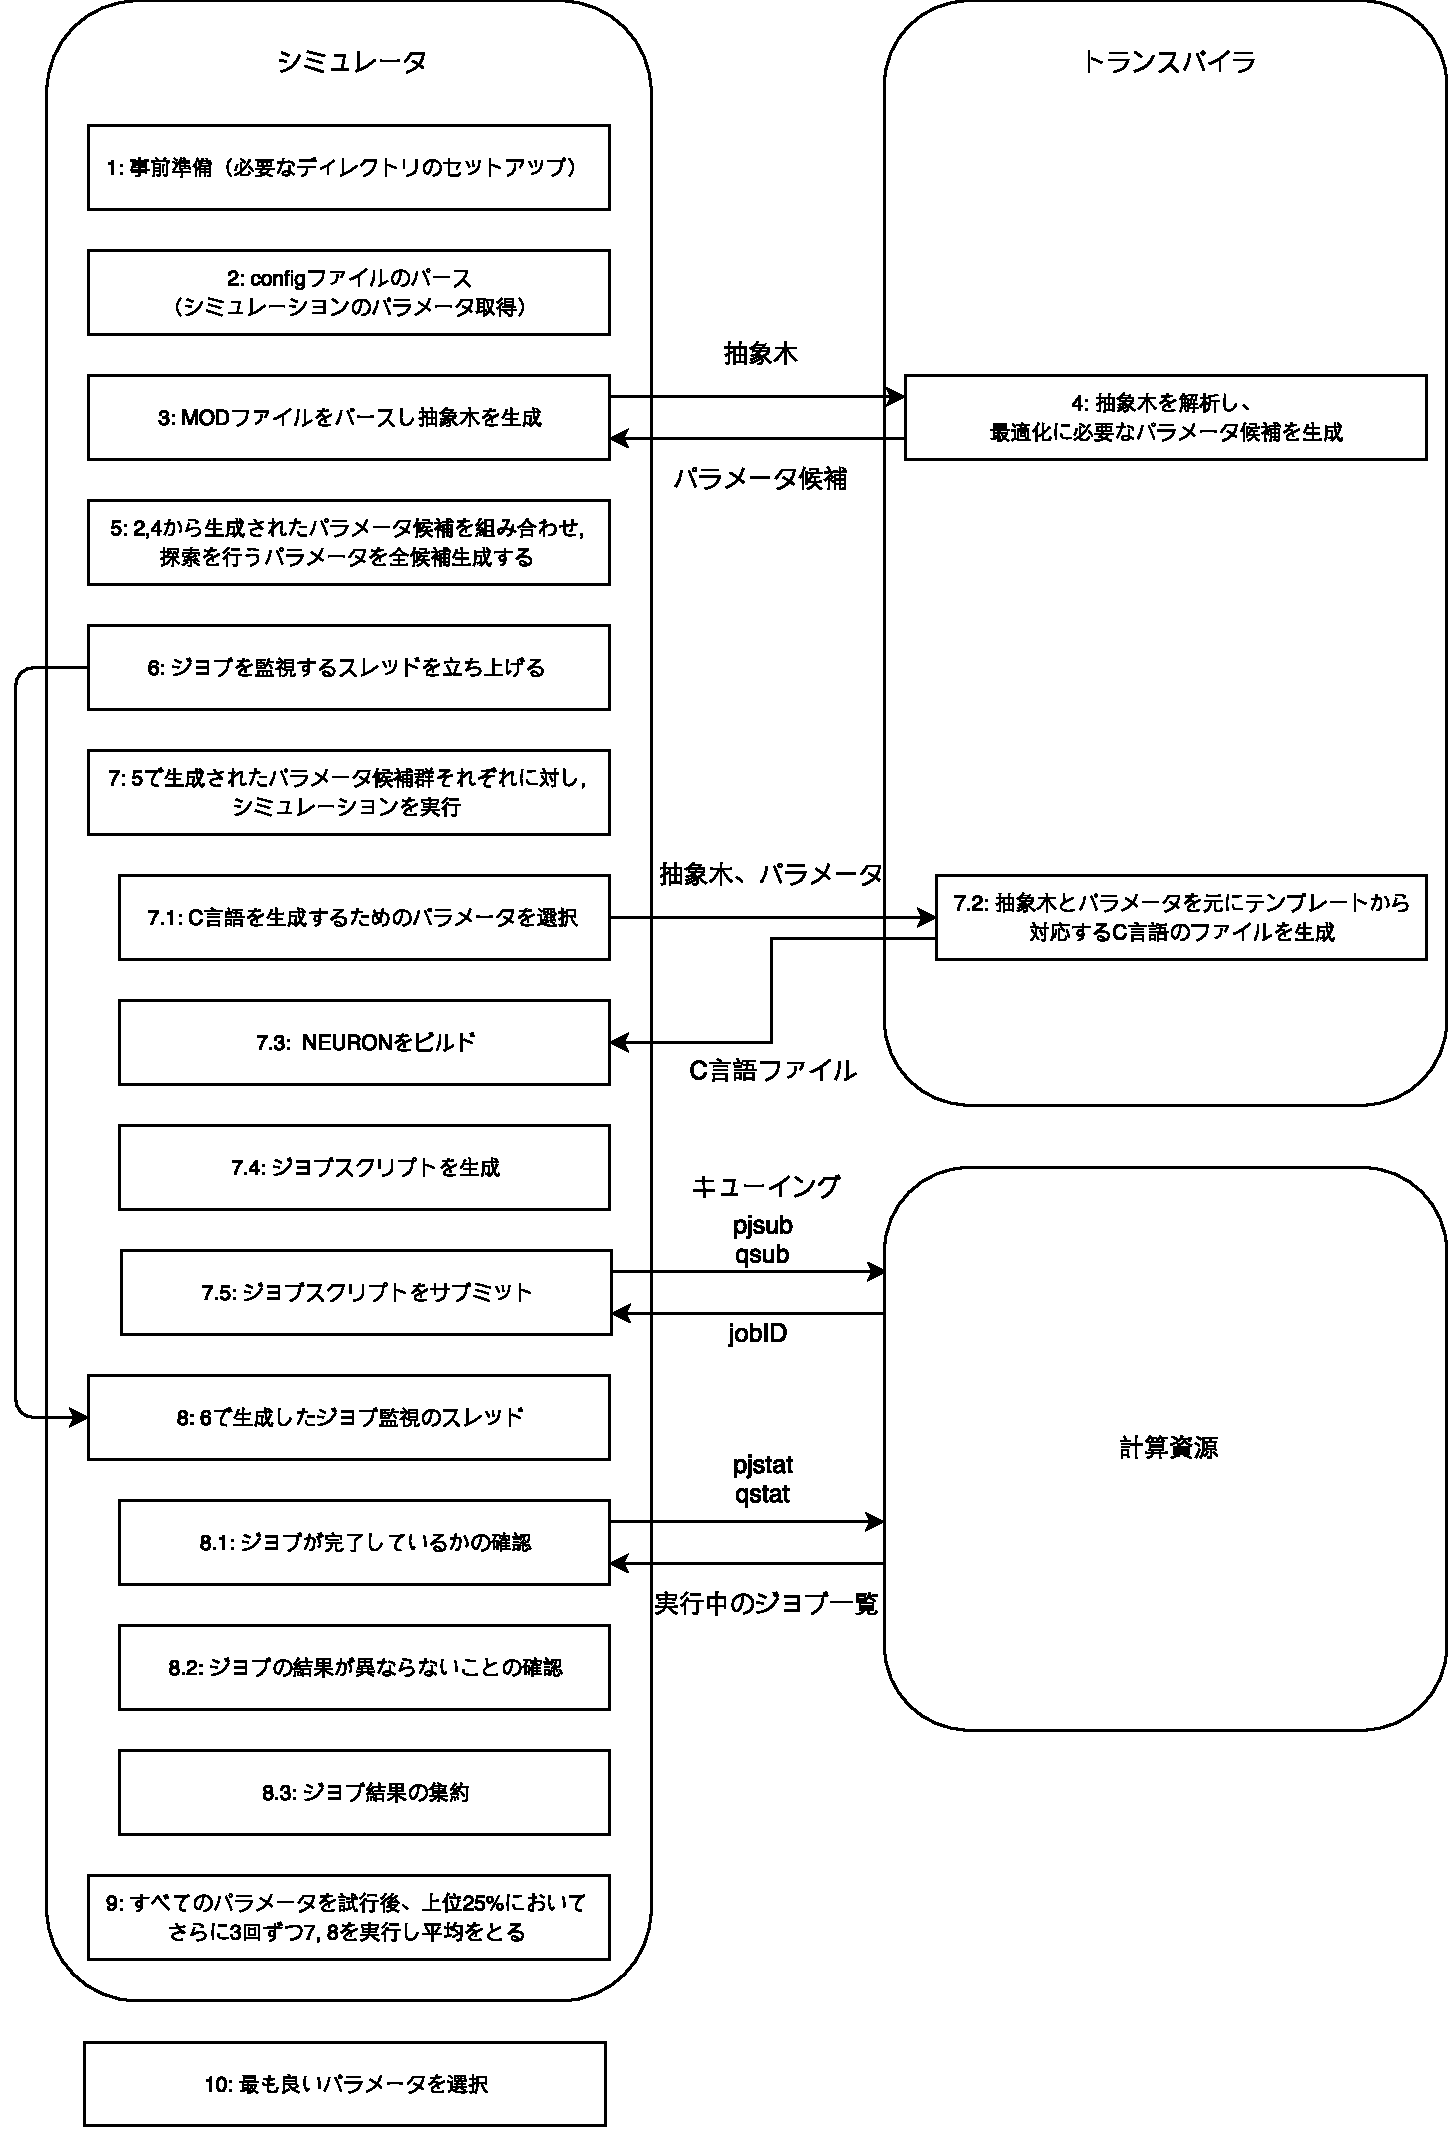
\includegraphics[width=18.0cm]{./images/Genie.pdf}
    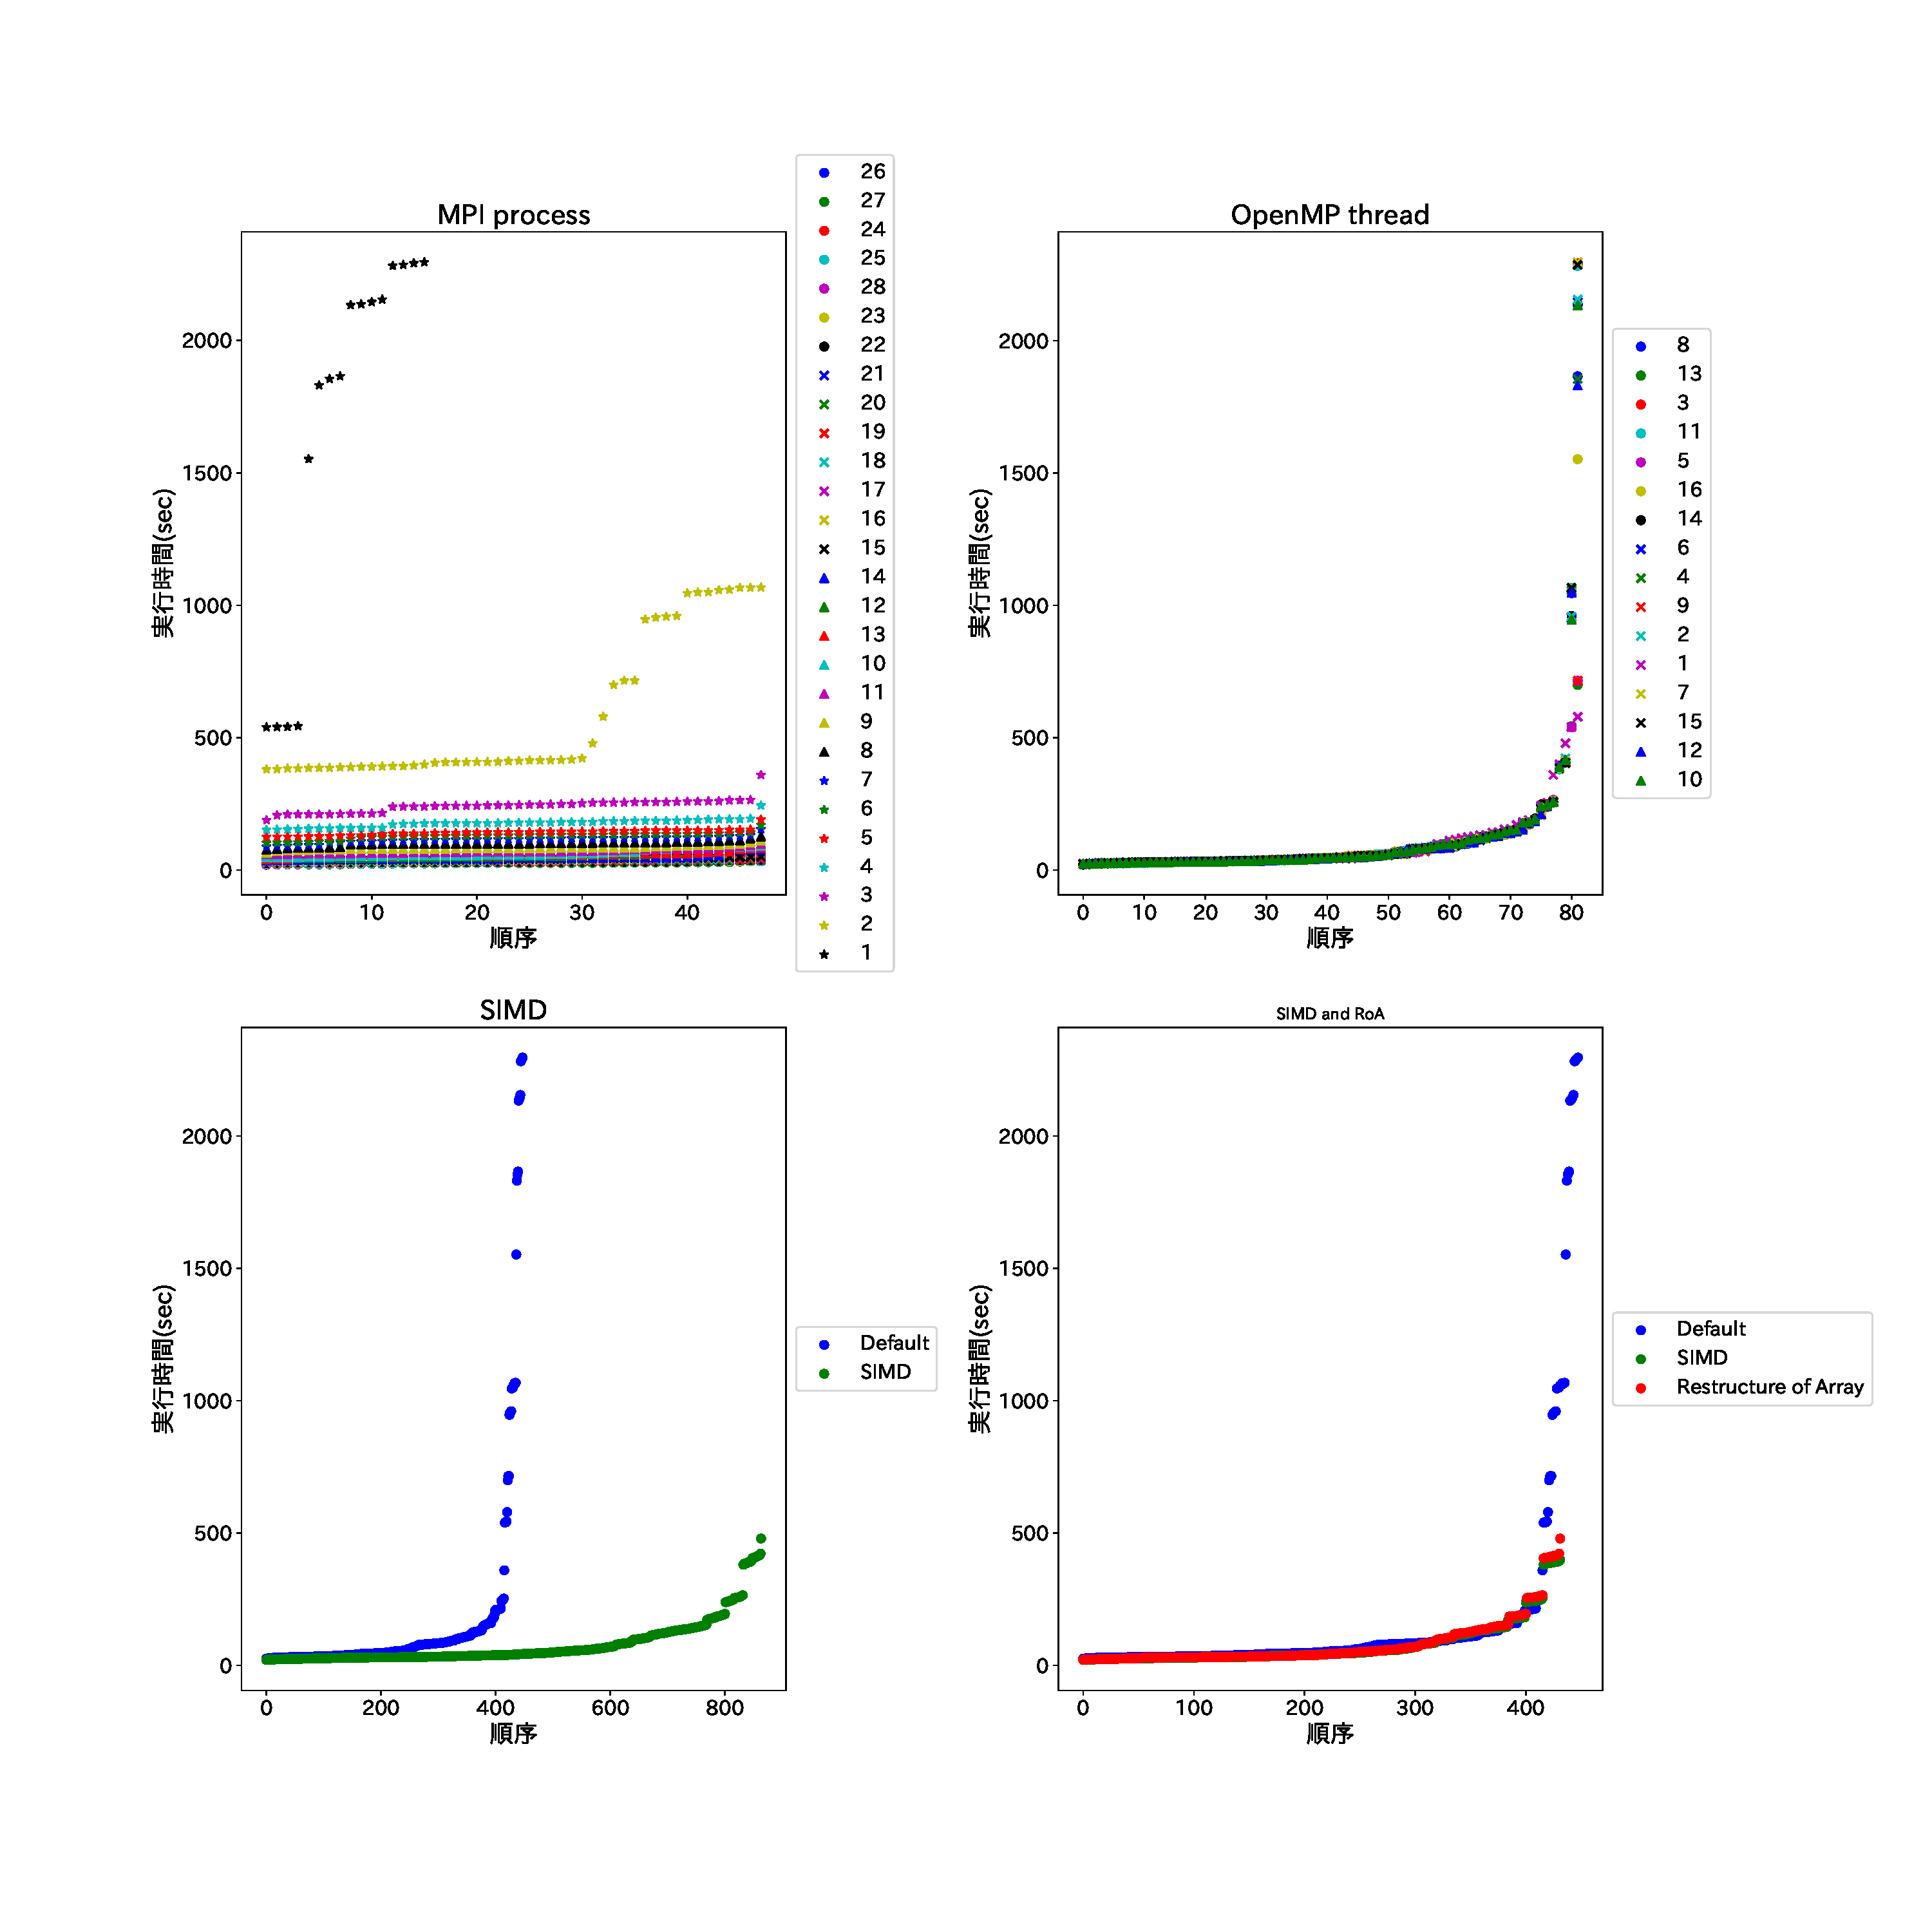
\includegraphics[width=1.2\textwidth]{./images/cluster-bench.pdf}
    \caption{クラスタ 小規模シミュレーション結果}
    \label{fig:cluster-bench}
 \end{center}
\end{figure}
一方で, この図では実行時間が短い部分が一部の非常に遅い実行時間に影響されて潰れてしまっている.
そこでパラメータと実行時間の関係を見るために, シミュレータでも利用している実行時間の上位25\%を用いる. その結果を図\ref{fig:cluster-bench-top25}に示す.\\
\begin{figure}[htb]
% h:here, t:top, b:bottom, p:page
 \begin{center}
%    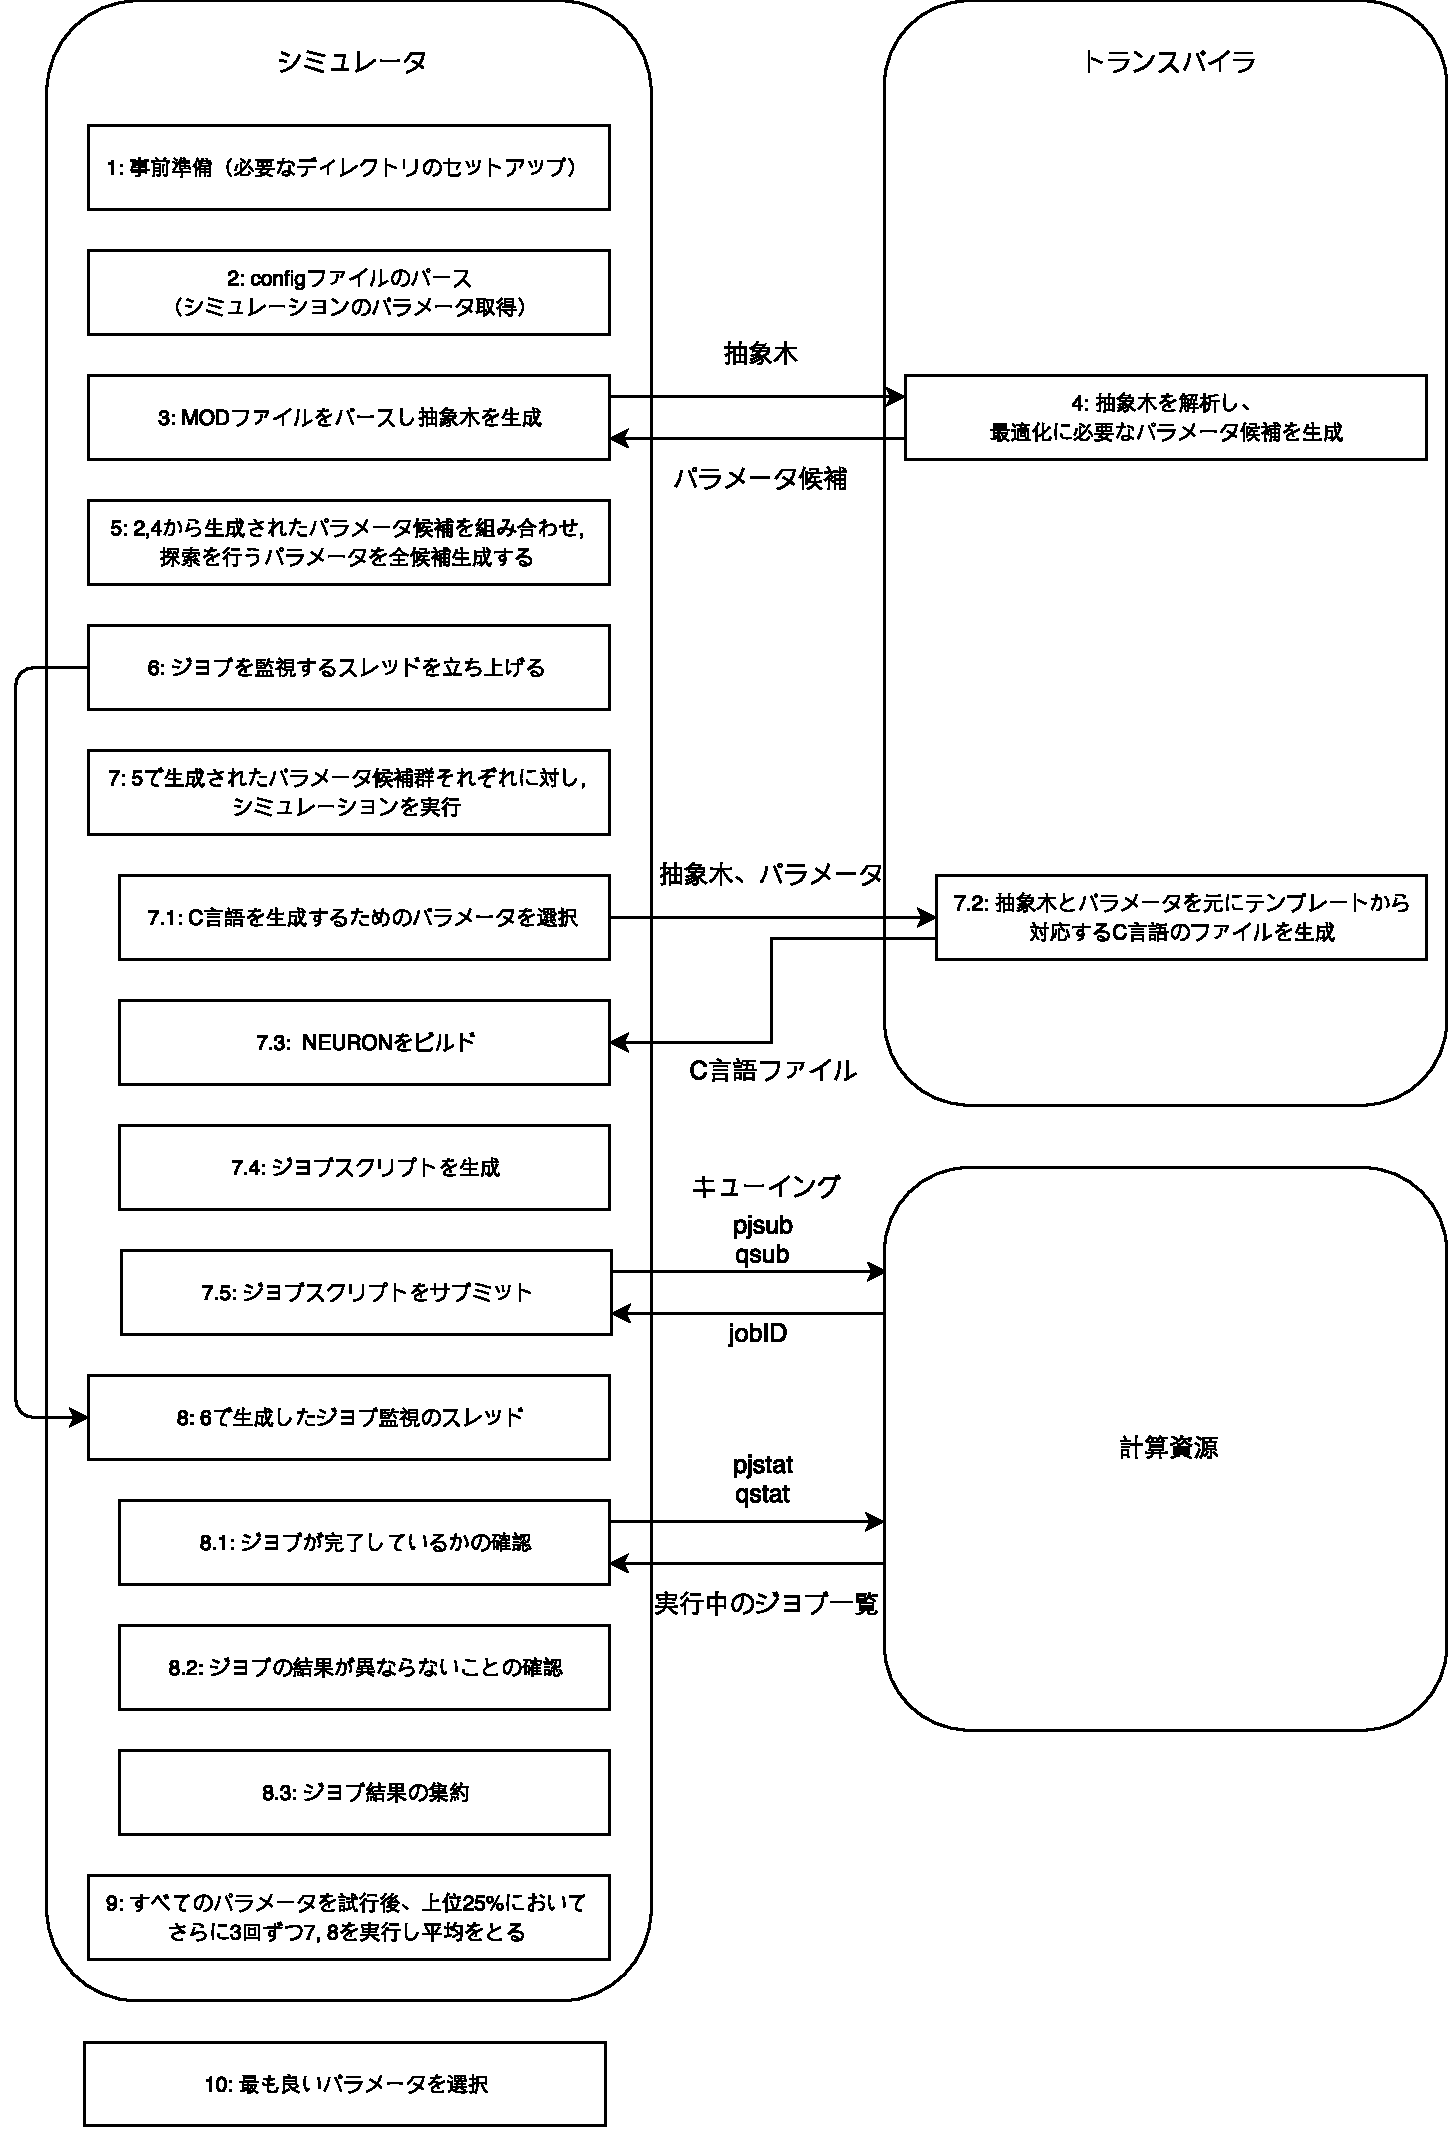
\includegraphics[width=18.0cm]{./images/Genie.pdf}
    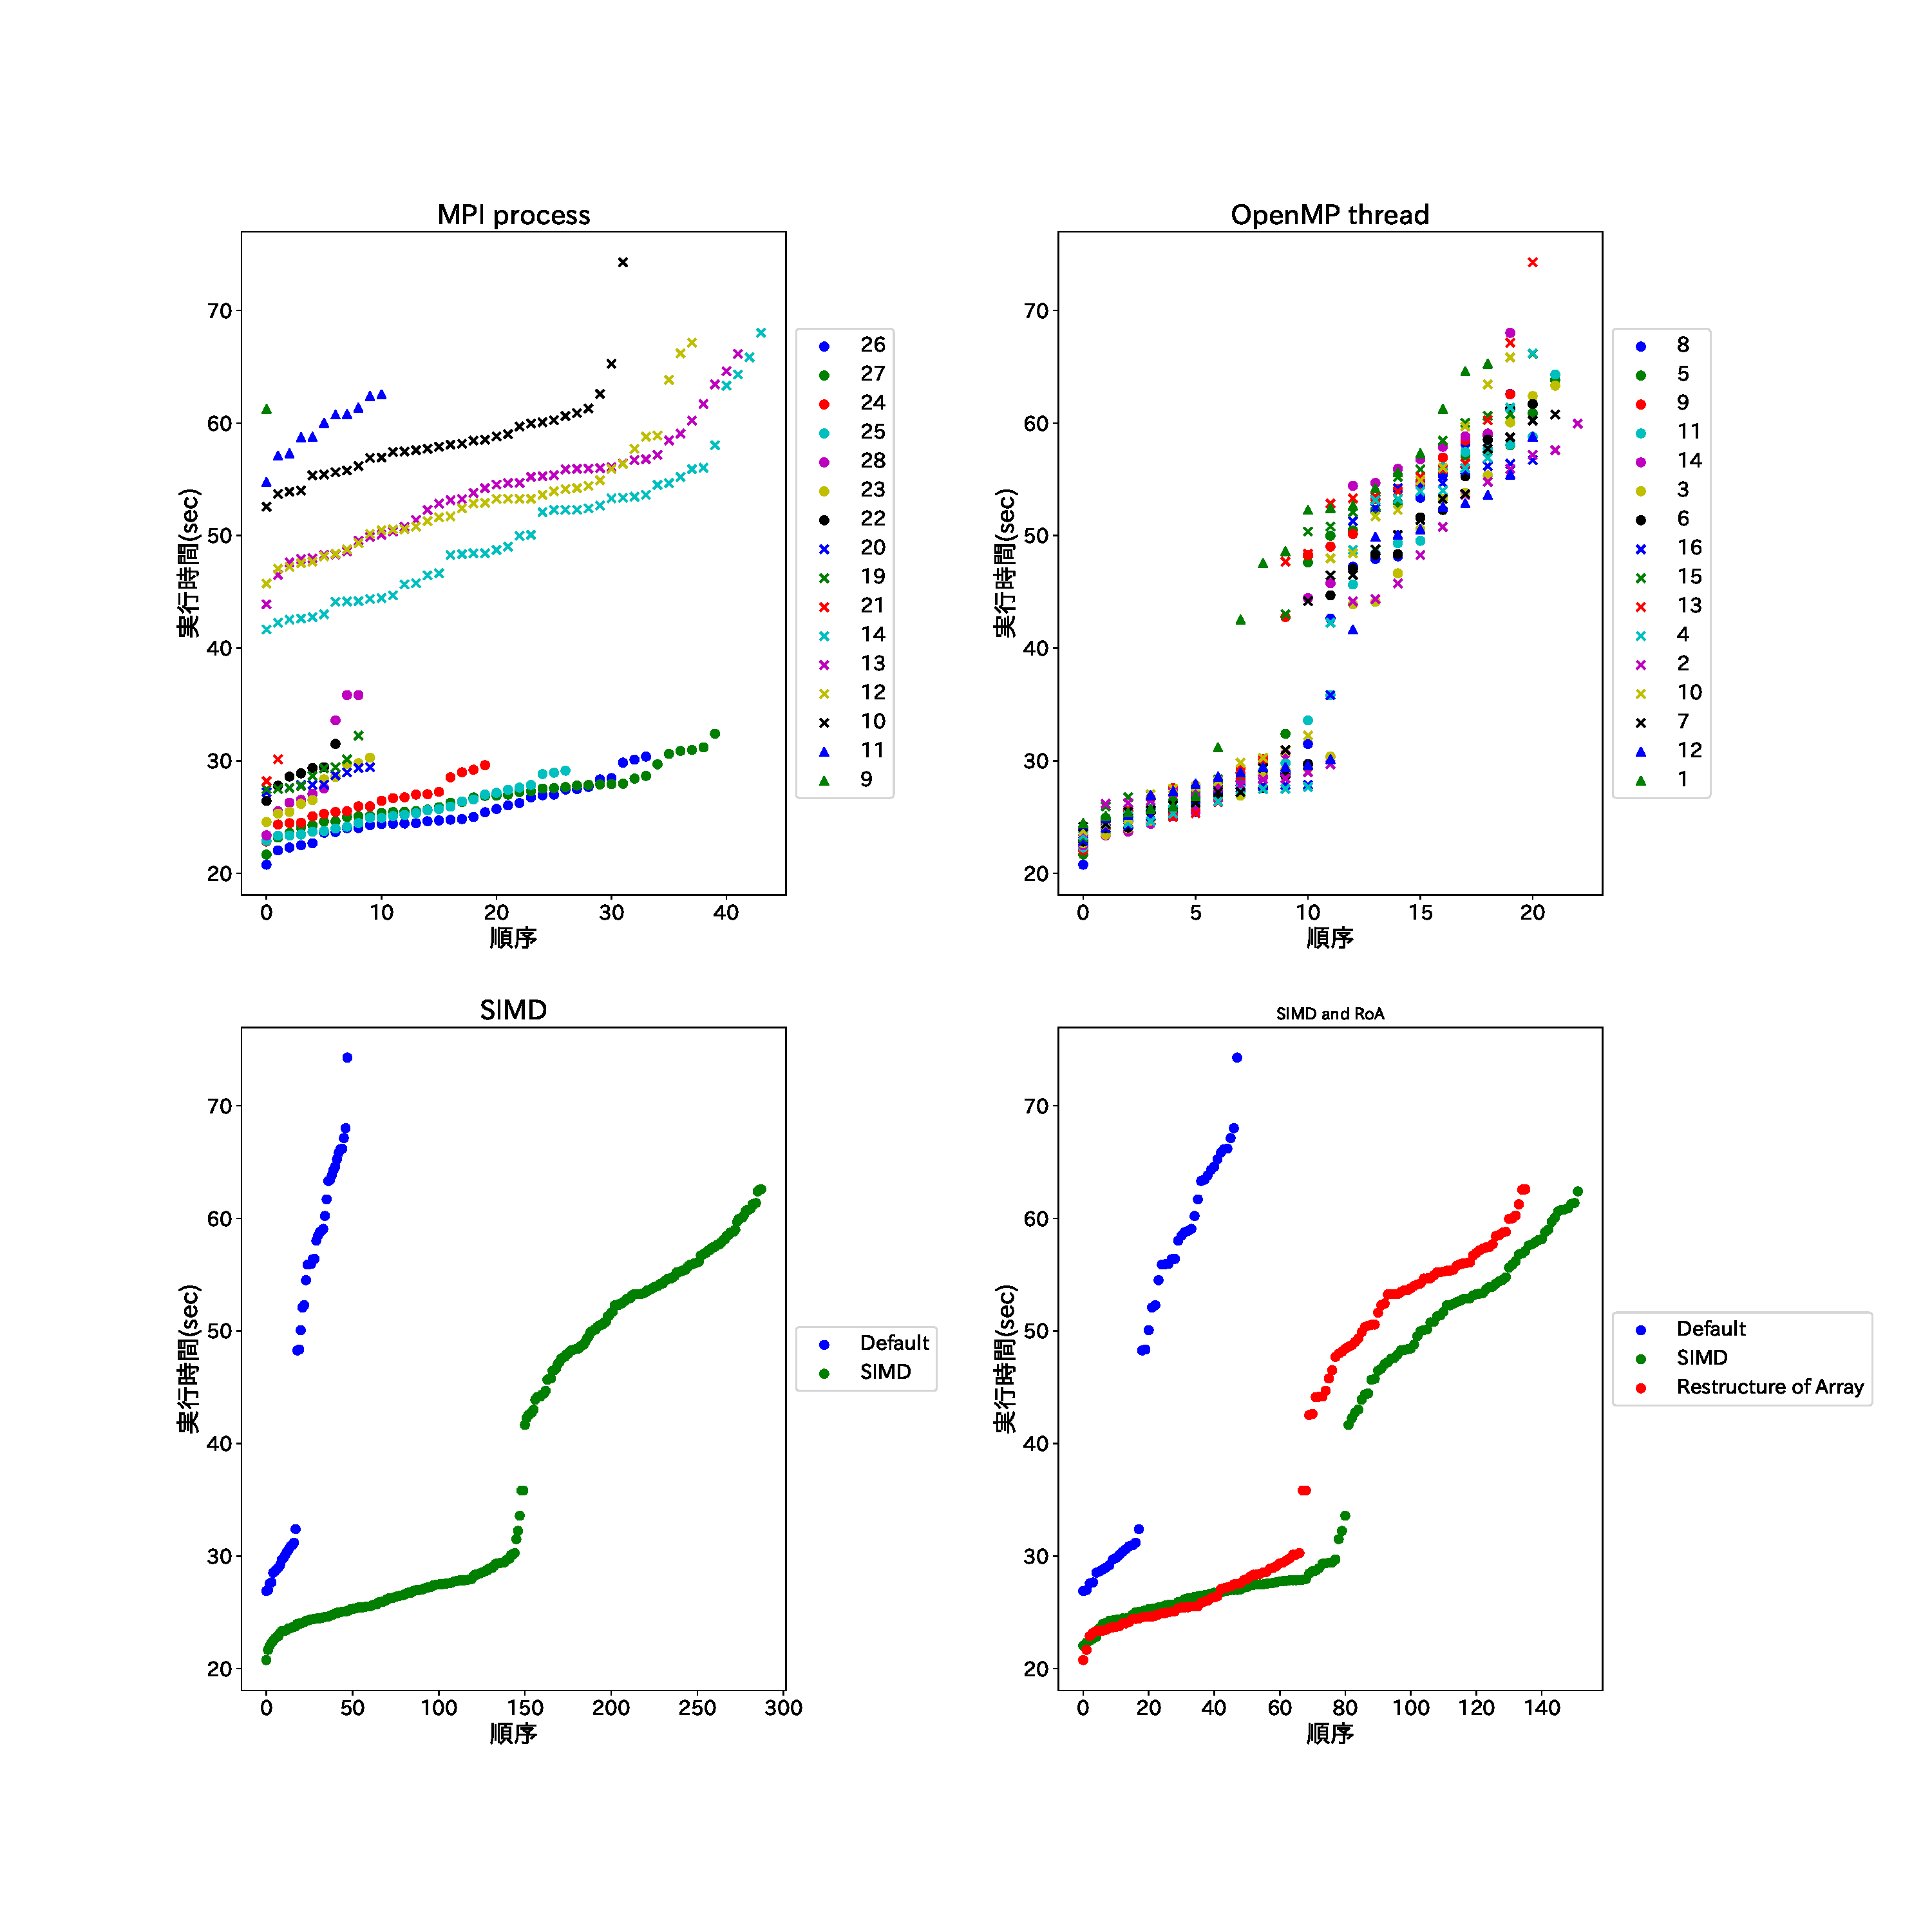
\includegraphics[width=1.2\textwidth]{./images/cluster-bench-top25.pdf}
    \caption{クラスタ 小規模シミュレーション結果 上位25\%}
    \label{fig:cluster-bench-top25}
 \end{center}
\end{figure}
図\ref{fig:cluster-bench-top25}では, まずMPIプロセス数に関してプロセス数が14以下のものとそれよりも大きいものの間で実行時間に大きな乖離があることがわかる.
本研究において求めるのは, 実行時間がその環境において最も早くなるパラメータ一組であり,
ここで求めたいものは5.2節以降に詳細にシミュレーションを行う意義のあるパラメータ候補であるため,
ためこのように明確に乖離が見られるパラメータは探索対象から除外することができる.\\
同様にして, 他の条件を固定した状態でパラメータの除外を行いパラメータによる有意差が生まれなくなるまで絞り込みを行った結果が図\ref{fig:cluster-bench-adjusted-final}である.\\
\begin{figure}[htb]
% h:here, t:top, b:bottom, p:page
\begin{center}
%    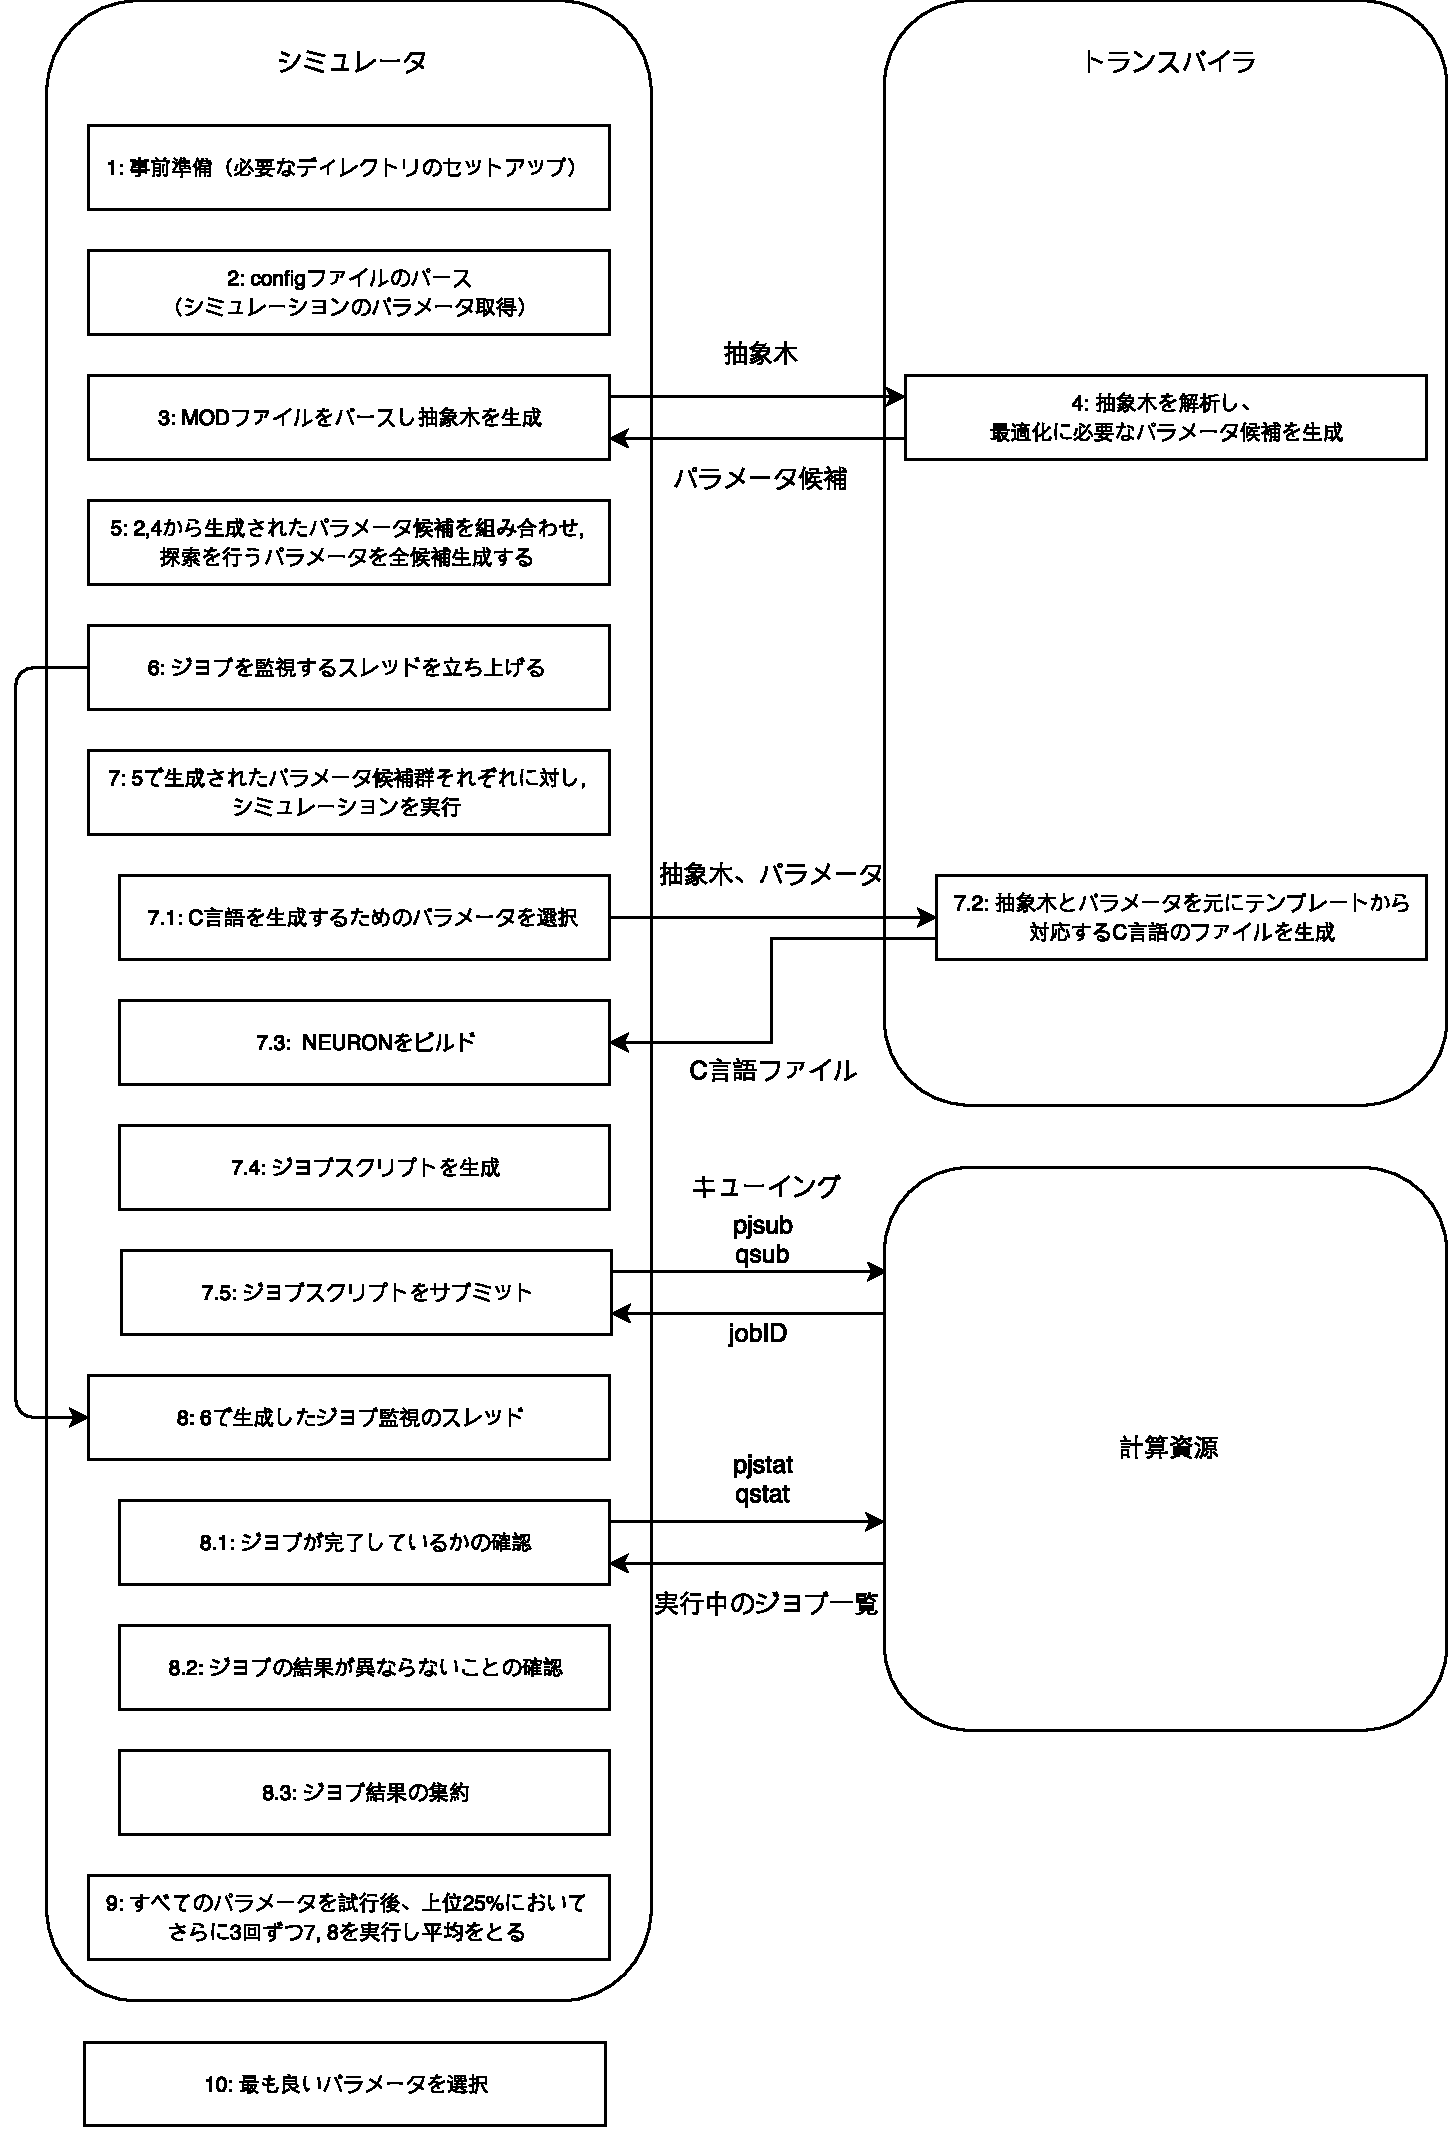
\includegraphics[width=18.0cm]{./images/Genie.pdf}
    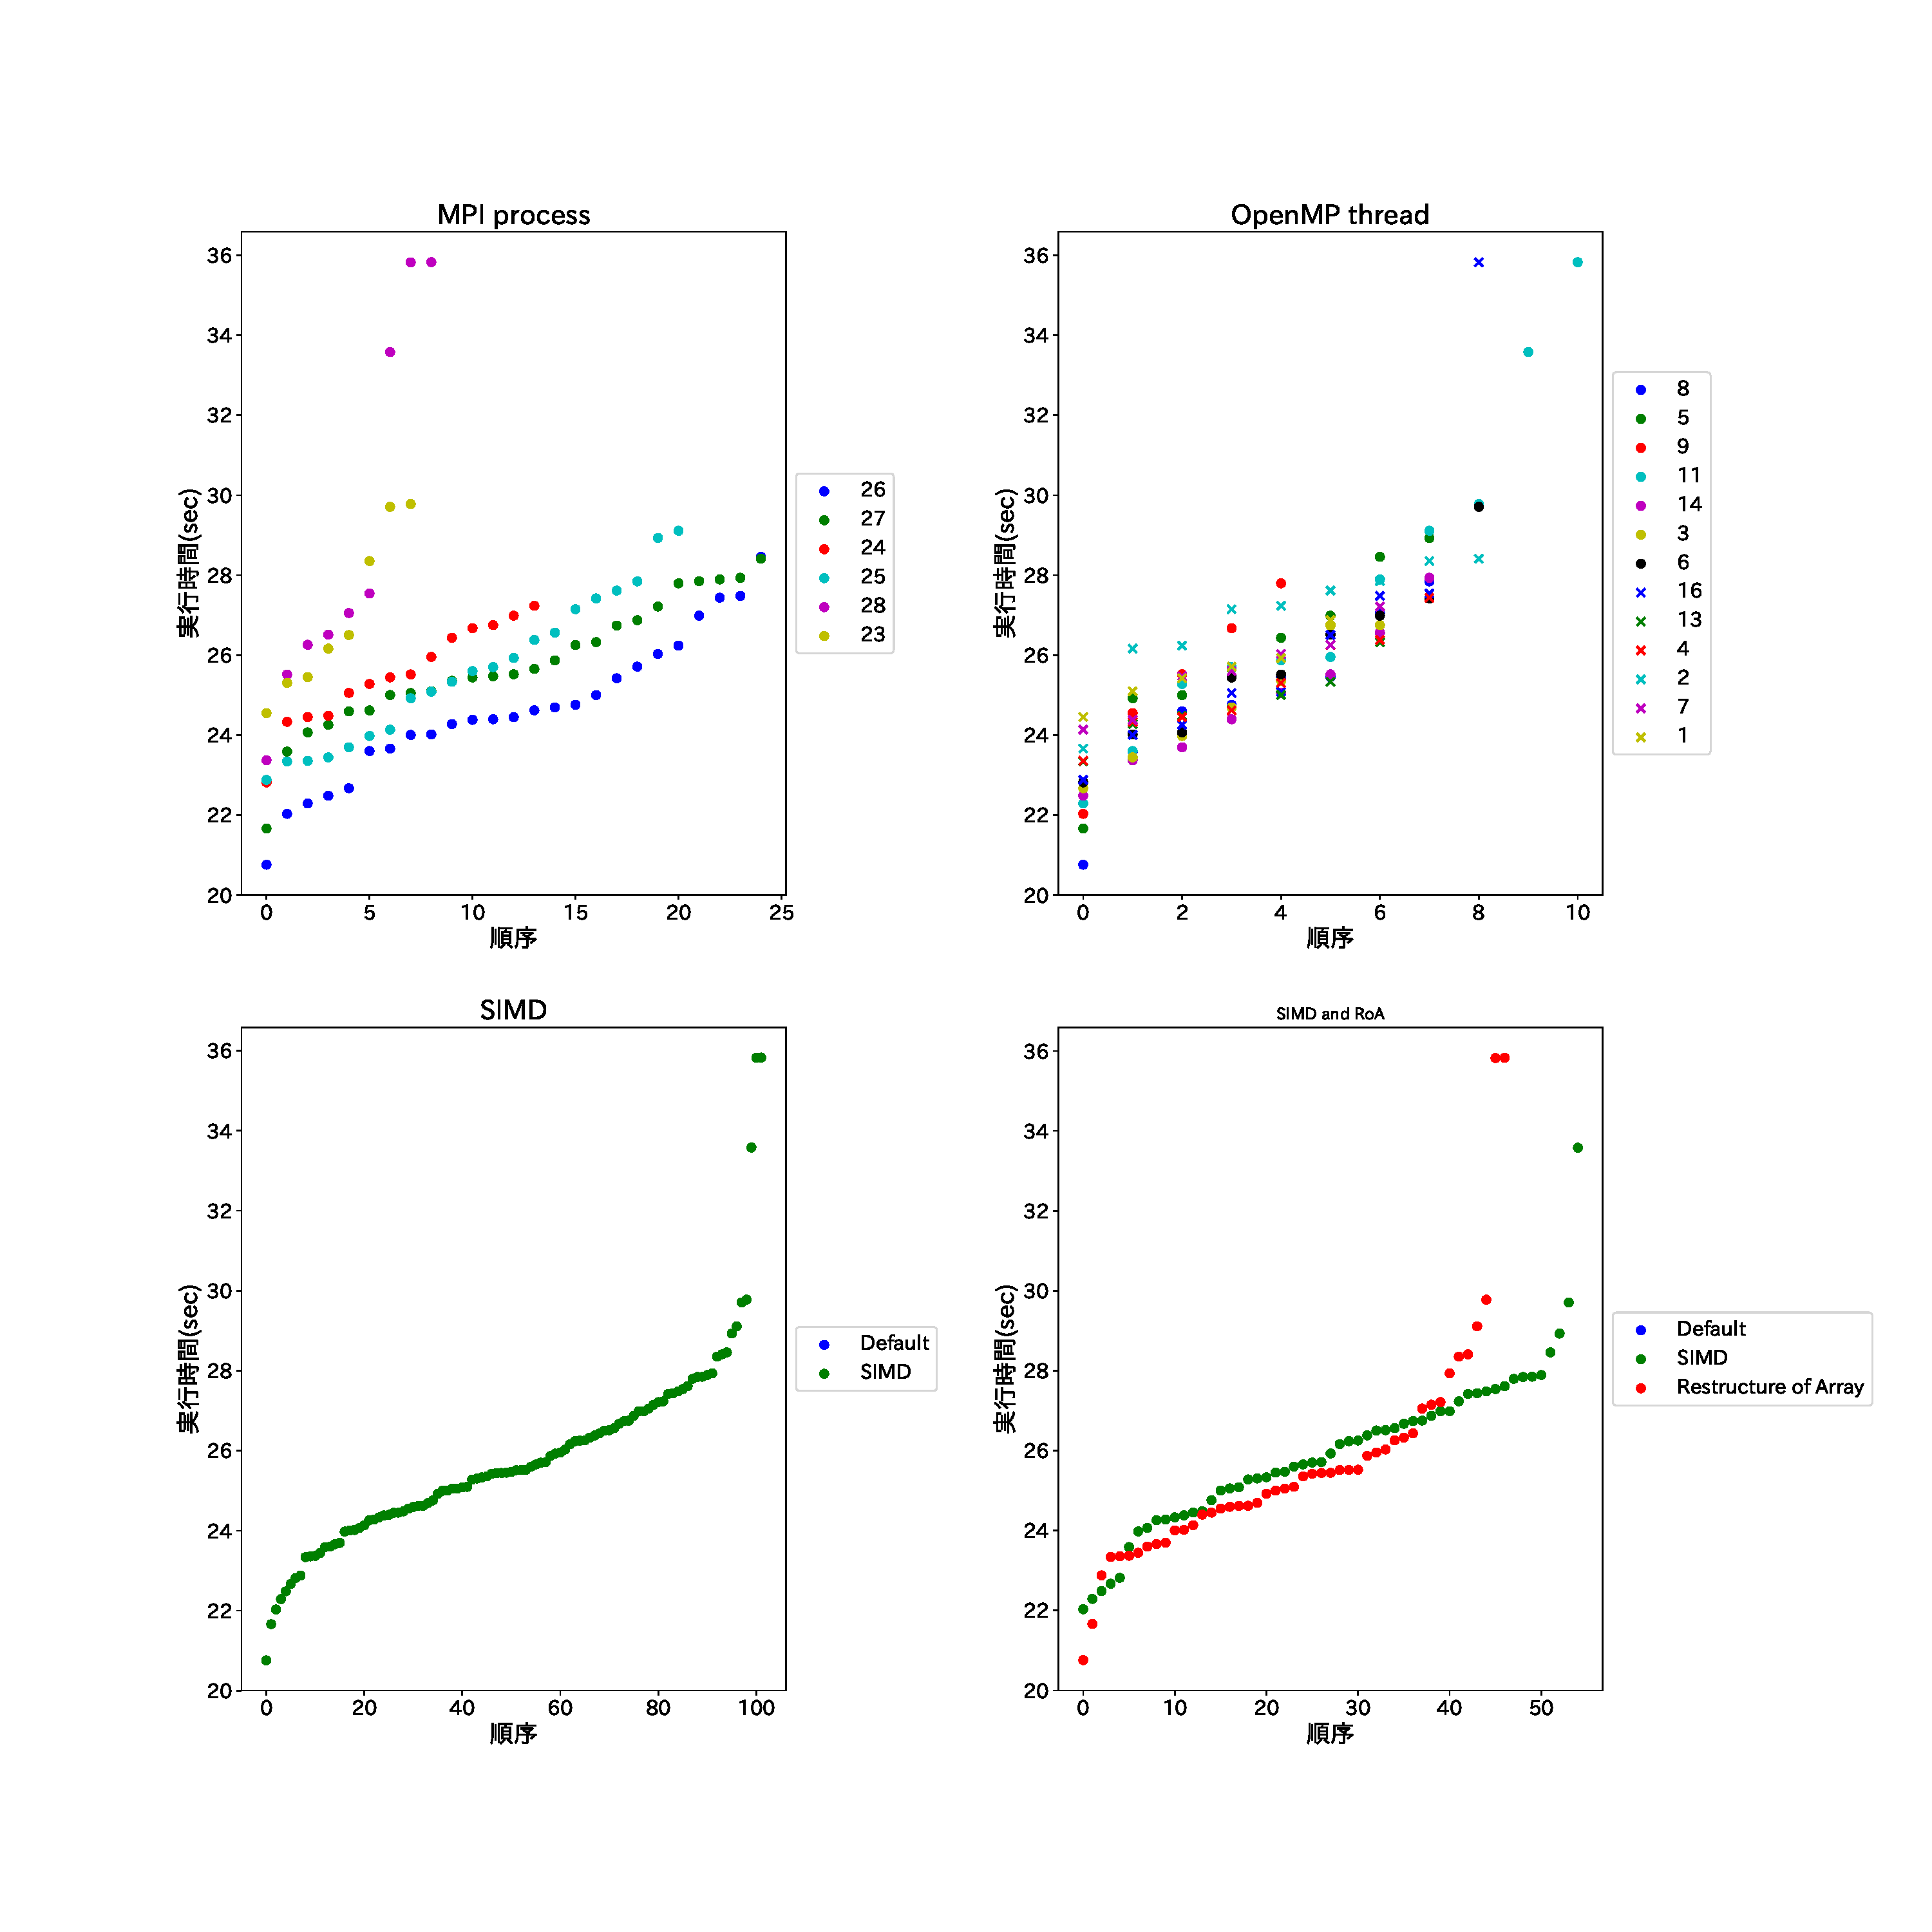
\includegraphics[width=1.2\textwidth]{./images/cluster-bench-adjusted-final.pdf}
    \caption{クラスタ 小規模シミュレーション結果 パラメータ絞り込み後}
    \label{fig:cluster-bench-adjusted-final}
\end{center}
\end{figure}
また絞り込みを行ったパラメータは次のようになる.\\
\begin{table}[htb]
  \caption {クラスタでの絞り込み後のパラメータ}
  \begin{center}
    \begin{tabular}{|c|p{12cm}|}
      \hline
      パラメータ & 値の範囲\\ \hline
      ノード数 & 1\\ \hline
      MPIプロセス数 & 23〜28\\ \hline
      OpenMPスレッド数 & [1, 2, 3, 4, 5, 6, 7, 8, 9, 11, 13, 14, 16]\\ \hline
      SIMD化 & 行う\\ \hline
      配列のくくり出し & 行う or 行わない\\ \hline
    \end{tabular}
  \end{center}
\end{table}

\clearpage
\subsubsection{京環境}
\begin{table}[htb]
  \caption {京でのパラメータ}
  \begin{center}
    \begin{tabular}{|c|p{12cm}|}
      \hline
      パラメータ & 値の範囲\\ \hline
      ノード数 & 8\\ \hline
      MPIプロセス数 & 1〜8\\ \hline
      OpenMPスレッド数 & 1〜16\\ \hline
      SIMD化 & 行う or 行わない\\ \hline
      配列のくくり出し & 行う(SIMD化を行っているならば) or 行わない\\ \hline
      シミュレーション時間 & 100ms\\ \hline
      神経細胞数 & 256\\ \hline
    \end{tabular}
  \end{center}
\end{table}
京においてもクラスタ同様パラメータの絞り込みを小規模シミュレーションを用いて行った.\\


\subsection{MPIプロセス数}

\subsection{OpenMPスレッド数}

\subsection{SIMD化}

\subsection{配列のくくり出し}

\subsection{最適化結果の比較}
